\documentclass[conference]{IEEEtran}

\usepackage{amsmath}
\usepackage{algorithm}
\usepackage{algorithmic}
\usepackage{graphicx}
\usepackage{cite}
\usepackage{array}
\usepackage{cases}
\usepackage{booktabs}
\usepackage{multirow}
\usepackage{epsfig}
\usepackage[TABBOTCAP]{subfigure}
\usepackage{esint}

\newtheorem{definition}{Definition}
\newtheorem{theorem}{Theorem}
\newtheorem{proposition}{Proposition}
\newtheorem{corollary}{Corollary}
\newtheorem{lemma}{Lemma}
\newtheorem{remark}{Remark}
\newtheorem{problem}{Problem}
\newcommand{\tabincell}[2]{\begin{tabular}{@{}#1@{}}#2\end{tabular}}


\hyphenation{op-tical net-works semi-conduc-tor}

\hyphenpenalty=5000
\tolerance=1200

\begin{document}

%\title{Alano: May You Discover Your Neighbors in Partially-Connected Networks}
\title{Alano: May You Discover Your Neighbors}

% author names and affiliations
% use a multiple column layout for up to three different
% affiliations

% conference papers do not typically use \thanks and this command
% is locked out in conference mode. If really needed, such as for
% the acknowledgment of grants, issue a \IEEEoverridecommandlockouts
% after \documentclass

% for over three affiliations, or if they all won't fit within the width
% of the page, use this alternative format:
%
%\author{\IEEEauthorblockN{Michael Shell\IEEEauthorrefmark{1},
%Homer Simpson\IEEEauthorrefmark{2},
%James Kirk\IEEEauthorrefmark{3},
%Montgomery Scott\IEEEauthorrefmark{3} and
%Eldon Tyrell\IEEEauthorrefmark{4}}
%\IEEEauthorblockA{\IEEEauthorrefmark{1}School of Electrical and Computer Engineering\\
%Georgia Institute of Technology,
%Atlanta, Georgia 30332--0250\\ Email: see http://www.michaelshell.org/contact.html}
%\IEEEauthorblockA{\IEEEauthorrefmark{2}Twentieth Century Fox, Springfield, USA\\
%Email: homer@thesimpsons.com}
%\IEEEauthorblockA{\IEEEauthorrefmark{3}Starfleet Academy, San Francisco, California 96678-2391\\
%Telephone: (800) 555--1212, Fax: (888) 555--1212}
%\IEEEauthorblockA{\IEEEauthorrefmark{4}Tyrell Inc., 123 Replicant Street, Los Angeles, California 90210--4321}}




\maketitle




\input{abstract}

\IEEEpeerreviewmaketitle

% Introduction
\section{Introduction}

%Paper Logic Flow
% P1-P2 Background
% P3-P6 motivation
% P7-P11 contribution
% P12 structure


% P1:    
% General background
% The situation&scenario our research applies to
Information and Communication Technology (ICT) equipment \cite{zeadally2012energy} has exploded 
on the scene in the last twenty years, leading to an obvious ascent of Internet-of-Things \cite{atzori2010internet},
such as wireless sensor networks[], mobile campus networks[], mobile gaming community[], etc.


% P2: 
% Why NB problem is related and important to the background in P1  
% Define what is neighbor and what is neighbor discovery problem
% A brief introduction of the existing works
Neighbor discovery is a fundamental step of constructing a wireless network, based on 
which the network can implement further applications such as routing and broadcasting.
The core target is for each node in the network to discover the nodes in its radio sensing range 
with one-hop communication, which are called neighbors. 
A number of existing methods \cite{dutta2008practical,kandhalu2010u,
bakht2012searchlight,sun2014hello,chen2015heterogeneous,
wang2015blinddate,qiu2016talk,mcglynn2001birthday,
vasudevan2009neighbor,you2011aloha,song2014probabilistic} have been proposed 
to deal with this issue, some of which are based on deterministic techniques while others
are probabilistic approaches.


% P3:
% Crucial problem:  existing network models are impractical
% What is the current network model
Unfortunately, there are some discrepancies between the current research network and the actual situation.
The deterministic methods deal with the neighbor discovery problem for two nodes and the
probabilistic approaches are designed for the networks where all the nodes can communicate with each other.


% P4:
% What is a practical network model and define what is a partially-connected network
In a large-scale and practical network, each node is only able to sense the 
nodes located nearby itself based on received signal strength \cite{wang2013gaussian}.  
We call this network connection structure as partially-connected networks.


% P5: 
% What issues will occur, if transferring the existing methods (mentioned in P2) to the partially-connected network
As for the deterministic approaches, when transferred to partially-connected networks,
they can not solve the collision issue when more than one neighbors are transmitting simultaneously. 
Relatively, the probabilistic approach can well deal with multiple nodes discovery but only consider
the network is fully-connected, the topology of which is a complete graph. 
Thus the probability adopted in these approaches can not be desirable.


% P6: 
% Summarize and highlight the crucial issue : partially-connected network and practical distribution
% Give the reason why it is import to take the distribution into consideration
To our best knowledge, no relevant researches have focused on neighbor discovery problem
in the partially-connected networks. More practically, in a wireless sensor network the distribution of 
sensors' deployment consequently plays a vital role in determining the intrusion detection capability of a sensor node.
Thus the distribution of the nodes in the network needs to be fully taken into 
consideration.

% P7:
% Our solution/contribution : we propose Alano algorithm based on the distribution of nodes for the partially-connected networks
In this paper, we propose Alano\footnote{Alano is the god of luck in Greek mythology }, 
a nearly optimal probability based algorithm to discover neighbors in partially-connected networks. 
As fully studied in \cite{wang2013gaussian} , the nodes in wireless sensor networks are likely to 
follow a uniform or a Gaussian distribution as showed in Fig. \ref{distribution}, 
depending on the specific network applications, which is taken in consideration of the proposed Alano algorithm.

 
 \begin{figure}[!t]
\centering
\subfigure[uniform distribution]{\includegraphics[width=1.7in]{./Figure/uniform.eps}}
\vspace{0.03in}
\subfigure[Gaussian distribution]{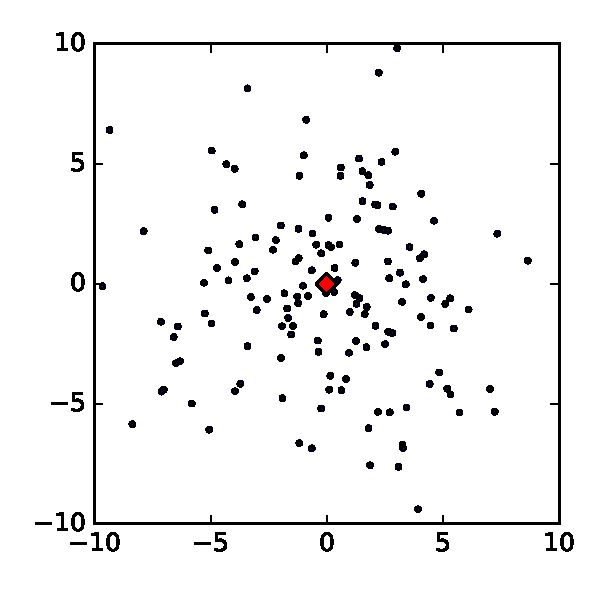
\includegraphics[width=1.7in]{./Figure/normal.eps}}
\caption{WSN deployments following uniform and Gaussian distribution.}
\label{distribution}
%\vspace{-0.2in}
\end{figure}


% P8: 
% A special type of partially-connected networks: energy-efficient network
In addition, among the partially-connected networks, there is a special 
type named energy-efficient network.
Wireless sensor network is a typical energy-efficient network that all the sensor nodes have to maintain 
strict power budgets to attain years of lifetime\cite{dunkels2011contikimac}.
Duty cycle mechanism, the fraction of time the radio is turned on, is 
utilized to raise the power-awareness of the nodes in the network.
Correspondingly, the neighbor discovery process 
needs adjustment to deal with the dilemma between 
a balance of energy-efficiency and low-latency.


% P9: 
% For energy-efficient networks, we propose RDS-Alano in global duty cycle scenario 
% and TP-Alano in the local duty cycle scenario.
For energy-efficient networks, we design deterministic methods
to align the wake-up time slot between the neighbors to achieve lower latency bound.
Specifically, We propose RDS-Alano algorithm for the global duty cycle scenario, where 
all the nodes share a identical duty cycle $\theta$ and TP-Alano for the
local duty cycle scenario where each node holds a distrinct duty cycle $\theta_i$. 


% P10:
% Simulation results support our high performance
Our simulation under the practical distribution of networks 
\cite{wang2013gaussian} shows the proposed Alano algorithm
holds significant strengths than the state-of-the-art methods,
based on the evaluation of speed, quality and scalability.
Alano achieves 31.35\% to 32.32 times lower latency
and has higher discovery rate during the whole course of neighbor discovery, 
with either global or local duty cycle in both uniform and Gaussian distribution.
When the number of nodes increases and the network becomes denser, 
Alano still keeps its high performance. 


% P11:
% Contribution summarize
The main contributions of this paper are summarized as follows:
\begin{itemize}
\item[1)] We model the distribution of node deployment with mathematical analysis 
and analyse the expectation number of neighbors of a node in uniform distribution and Gaussian
distribution.
\item[2)] We propose Alano, a low-latency strategy to achieve neighbor discovery process
in a partially-connected network.
\item[3)] We propose a Relaxed DifferenceSet based Alano algorithm (RDS-Alano) 
to achieve low-latency neighbor discovery process in the global duty cycle scenario. 
\item[4)] We propose a Traversing Pointer based Alano algorithm (TP-Alano) 
achieve low-latency neighbor discovery process in the local duty cycle scenario. 
\end{itemize}


% P12:
% Remaining structure
The remainder of the paper is organized as follows.
The next section highlights some related work and 
puts forward some serious problems. 
Some notion definitions and the system model are given in Section
\ref{sectionmodel}. 
We analyse the node's expectation number of neighbors and 
propose Alano algorithm in \ref{PCN} as a foundation.
Section \ref{EEN} describes the RDS-Alano algorithm for global
duty cycle scenario and TP-Alano algorithm for local duty cycle scenario
respectively in energy-efficient networks.
We have conducted extensive simulations, and the results are shown in Section
\ref{Evaluation}. Finally, we conclude the paper in Section
\ref{Conclusion}.



% Related Work
\section{Related Work}
\label{RW}

%Introduce the representative existing algorithms and the weakness.

%cite
%deterministic:
%BlindDate #wang2015blinddate
%Disco #dutta2008practical
%Hello #sun2014hello
%Searchlight #bakht2012searchlight
%Talk More Listen Less  #qiu2016talk
%Todis\&Hedis #chen2015heterogeneous
%U-Connect  #kandhalu2010u
%probabilistic:
%Birthday #mcglynn2001birthday
%ALOHA-like09 vasudevan2009neighbor
%ALOHA-like11 2011 #you2011aloha
%PND #song2014probabilistic
%others
%Normal Distribution #wang2013gaussian





Neighbor discovery problem has raised a great deal of attention of scholars \cite{sun2014energy}. 
A number of neighbor discovery methods have been proposed in the past decade.
Technically, these approaches can be classified into two categories, probabilistic and deterministic. 

In the deterministic methods \cite{dutta2008practical,kandhalu2010u,
bakht2012searchlight,sun2014hello,chen2015heterogeneous,
wang2015blinddate,qiu2016talk}, some mathematical techniques, such as
co-primality, quorum system, etc., are utilized to promote the discovery performance.
The deterministic methods holds an obvious advantage that they
can achieve neighbor discovery process within a bounded time latency.

Nevertheless, there exists some crucial weak points in the deterministic algorithm.
Firstly, Disco \cite{dutta2008practical} proposes a discovery protocol that
each node has a capability to send a beacon at both beginning and end of
an active slot, which is widely adopted by the later algorithms such as
SearchLight \cite{bakht2012searchlight}, BlindDate \cite{wang2015blinddate}
and Hello \cite{sun2014hello}, Nihao \cite{qiu2016talk}. It is quite an efficient way for two nodes to discover
each other within an ideal time latency. However,  they do not solve the collision 
issues when receiving packages from multiple neighbors. Furthermore, when they are 
extended for multiple nodes, only sending a beacon to discover the neighbors is 
totally insufficient. A node needs to send a complete package containing all its information,
otherwise the neighbor can not  identify which neighbor the beacon belongs to[][][].
Thus a complete time slot is necessary for a node to transmit a package or listen to 
the channel to receive a package.

Another category is probabilistic methods \cite{mcglynn2001birthday,
vasudevan2009neighbor,you2011aloha,song2014probabilistic}. These
approaches utilize probability techniques to promote the randomness 
to discover the neighbors. Different from the deterministic algorithms, 
this kind of method shows an significant strength in the multiple nodes scenario. 
Relatively, probabilistic methods only present an expectation discovery latency and 
can not guarantee a latency bound in the worst case.
In addition, almost all the existing methods consider the network is fully-connected,
the topology of which is a complete graph. Deploying a fully-connected network 
in a large-scale area is technically impractical 
due to the limited sensing range of devices communication.
How far the other nodes can be detected as a neighbor for a mobile equipment  
depends on criterion such as the received signal strength.
From our analysis and simulations, 
they have a poor performance in the partially-connected networks, which is more 
practical in the reality world.

To the best of our knowledge, neighbor deterministic nor probabilistic methods are designed for
partially-connected networks. In this paper, we present a low-latency, energy-efficient 
neighbor discovery algorithm for partially-connected networks.

The proposed RDS-Alano and TP-Alano in this paper are a combination of both two categories.
We compare our proposed algorithm with both deterministic and probabilistic algorithms. 
Particularly as mentioned above, the deterministic approaches need some adjustment 
when transferred to partially-connected networks. Details will be introduced in Section \ref{Evaluation}






\vspace{3mm}
(Note : Introduction and Related Work are expected to be 2 pages)

%\section{System Model and Problem Formulation}
\section{Preliminaries}
\label{sectionmodel}

In this section, we first describe the network and node model.
Then we formulate the Neighbor Discovery problem formally.  

\subsection{Network and Node Model}

%distribution and networks
In a network, the location of the nodes are likely to obey uniform distribution[][],
Gaussian distribution[][] or other combinatorial distributions.

In reality, since the network is deployed in a vast area, each node 
has a capacity to sense a fraction of nodes within its sensing range.
These networks are defined as \emph{Partially-Connected Networks}.

Among the partially-connected networks, there is a particular type called \emph{Energy-Efficient Networks}.
A typical one of energy-efficient networks is the wireless sensor network.
The wireless sensor network consists of a number of sensors distributed separately in a target area.
The deployed sensor nodes keep their most time in sleep pattern to avoid quick energy consumption 
and wake up timely to work on duty.


When a node wake up on a time slot, it can turn to either the transmitting state or listening state. 
\begin{itemize}
\item \textbf{Transmitting state}. A node turn to transmitting state will broadcast a package containing its own identify 
information to all neighbors.
\item  \textbf{Listening state}. A node turn to listening state will monitor the frequency channel to collect its neighbors' packages.
However collision will occur when two or more neighbor nodes transmit concurrently and thus no valid information will be gathered
\end{itemize}
Transiting between the states only costs little time, compared to one complete time slot.

In our model, we denote the node set in the network as $U = \{u_1,u_2,...,u_N\}$.
Time is divided into slots of equal length $t_0$, 
which is sufficient to finish  one communication process
(transmit or receive a piece of package). In each time slot, 
a node transform its pattern according to a pre-defined duty schedule.


\begin{definition}
\textbf{Duty Schedule} is a pre-defined sequence $S=\{s^t\}_{0\leq t<T}$ of period $T$ and
$$ s^t=\left\{
\begin{aligned}
S  & & & {Sleep}\\
T  & & & {Transmit}\\
L  & & & {Listen}\\
\end{aligned}
\right.
$$
\end{definition}

 Each node construct its own duty schedule according to a specific strategy and repeats it
 until finding all the neighbors. Since the waking-up duration has a significant affect on the battery's lifetime, 
 duty circle is utilized to restrict the energy consumption.

\begin{definition}
\textbf{Duty Circle} represents the fraction of one period T where a node turns its radio on. It can be formulated as:

$$\theta=\frac{|\{t: 0\leq t<T, s^t \in \{T,L\}\}|}{T}.
$$
  
\end{definition}

A homogeneous energy-arrangement case is that all the nodes
in the network share a common global duty circle $\theta$,
while each nodes holding a local duty circle $\theta_i$ is 
a heterogeneous


\subsection{Problem Definition}

We consider a partially-connected network, 
where two nodes are neighbors if they locate within the radio range of each other. 
A  symmetric matrix $M_{N\times N}$ is used to record the neighboring relations as:

$$ M_{i,j}=\left\{
\begin{aligned}
1  & & & & & & {connected}\\
0  & & & & & & {disconnected}\\
\end{aligned}
\right.
$$

Each node follows its duty schedule to achieve neighbor discovery. In a synchronous scenario,
nodes start their neighbor discovery process at the same time, while in a asynchronous  scenario
all nodes start at different time slots. We focus on the asynchronous case while still applicable for the
synchronous situation.

 
Notice that the neighbor discovery process is not bidirectional, which means any pair of neighbors 
need to find each other separately. The time slots within which a node $u_i$ find one of its neighbors $u_j$ can be formulated 
as $L(i,j)$. Then we define the discovery latency that node $u_i$ discovers all neighbors as:
\begin{definition}
\textbf{Discovery Latency} of node $u_i$ is the time to discover all neighbors:
$$L(i) = \max_{j:M_{i,j}=1} L(i,j).
$$
\end{definition}

Thus the neighbor discovery problem can be formulated as:
%@@@to be modified
\begin{problem}
For a node $u_i$ with its neighbor set $S = \{u_{i1},u_{i2},...u_{ij},...\}$, 
design a strategy to construct a duty schedule, which satisfies
$\forall$ neighbor nodes $u_{ij}$ :
$$
\exists t \ s.t. :  \quad
S_i(t) = L ,
S_{ij}(t) = T,
\forall k \neq j : S_{ik}(t) \in \{L, S\}.
$$

\end{problem}
%@@@

\begin{figure}[!h]
\centering
\subfigure[The topology of a wireless sensor networks ]{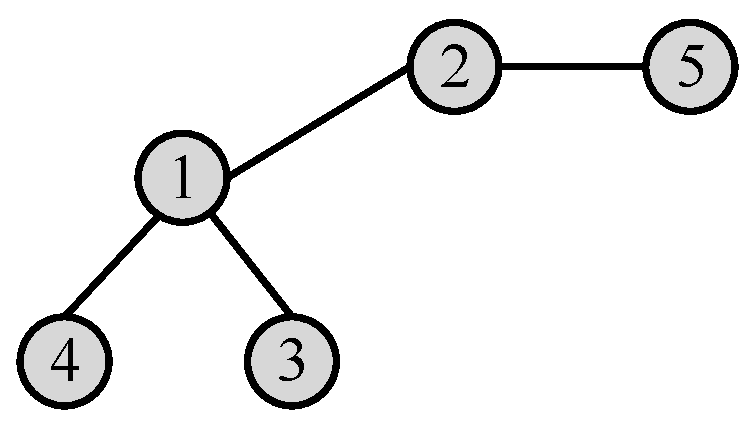
\includegraphics[width=1.65in]{./Figure/topology.eps}}
\vspace{0.03in}
\subfigure[Neighbor discovery process]{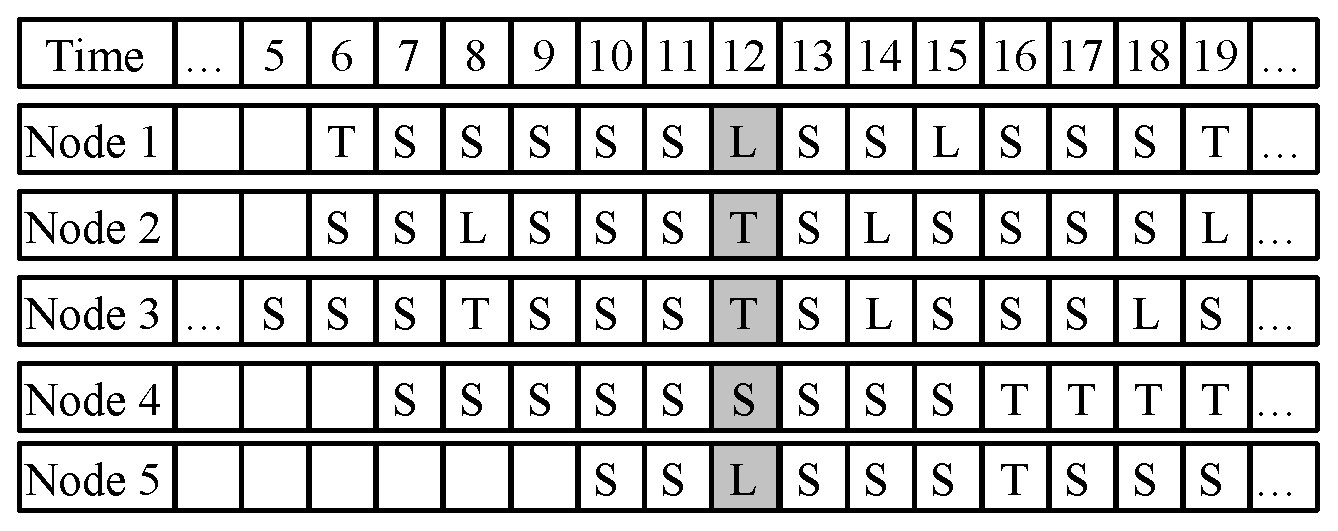
\includegraphics[width=2.8in]{./Figure/NBexample.eps}}
\caption{An example of neighbor discovering process. S, T and L represents Sleep pattern, 
Transmitting state and Listening state in wake-up pattern respectively.}
\label{NDexample}
%\vspace{-0.2in}
\end{figure}

An example of neighbor discovery process is given in Fig.\ref{NDexample}. 
Fig.\ref{NDexample}(a) shows the topology of a partially-connected 
wireless sensor network, which consists of $5$ sensor nodes. 
Fig.\ref{NDexample}(b) describes the neighbor discovery process 
in the asynchronous scenario, as we can see the nodes 
start their process at different time slot. The duty schedule of 
node $1$, for example, is $S_1 = \{ 1, 0, 0, 0, 0, 0, 1, 0, 0, 1, 0, 0, 0, 1, ... \}$.  
At time slot $12$, node 5 find its neighbor node $2$ while node $1$ 
could not find node $2$ due to a collision from its another neighbor node $3$. 





\section{Alano Algorithm for a large-scale Network}
%\section{Large-Scale Networks}
\label{PCN}

%Expectation			#meester1996continuum
%Geometric distribution	#Motwani1995Randomized
%Temperature 			#flammini2007real

%background and instances
In large-scale networks, nodes are not fully-connected and thus communications may fail due to concurrent transmissions. 
When we do not consider the energy constraints of nodes, we propose a nearly optimal algorithm for a large-scale network, which implies $\theta_i = 1$ for all node $u_i$.
Suppose the locations of nodes obey some distribution, we propose Alano algorithm and analyze its performance for two common used distribution (uniform distribution and Gaussian distribution).

\subsection{Alano Algorithm}
Suppose the locations of nodes obey some distribution and each node $u_i$ is aware of its position coordinates $(x_i, y_i)$.
Then $u_i$ could compute its local density by the following general function: % \cite{meester1996continuum, wang2015connectivity}.
$$f(x,y)=
\begin{cases}
\varphi(x,y)& (x,y)\in D\\
0& (x,y)\notin D
\end{cases}$$
where $(x,y)$ is a position coordinate, and $D$ is the network covering area.
%For each node $u_i$ with position $(x_i,y_i)$, T
Denote the range of $u_i$'s neighbors' positions as $R_i$,  and any neighbor with coordinates $(x,y) \in R_i$ suits:
$$
(x-x_i)^2+(y-y_i)^2 \leq \Delta^2
$$
where $\Delta$ is the communication range. Then, node $u_i$'s expected number of neighbors (denote as $\widetilde{n_i}$) is:
$$
\widetilde{n_i} = N\iint_{R_i} f(x,y)\,dx\,dy - 1.
$$

In a large-scale network, we ignore the boundary area of the network.  %and assume nodes in the network are of an enormous quantity. 
Note that, when the network covering area $D$ is much larger than the area $R_i$ of node $u_i$, we have:
\begin{equation}
\label{eqnNB}
\widetilde{n_i} \simeq N\pi \Delta^2 \varphi(x_i,y_i).
\end{equation}


%Alano
We present \textbf{Alano}, a randomized algorithm for node $u_i$ in Alg. \ref{Alano}.
By computing the expected number of nodes, $u_i$ turn to be in transmitting state or listening state according to the generated probability in Line \ref{pro}.


\begin{algorithm}
\caption{Alano Algorithm}
\label{Alano}
\begin{algorithmic}[1]
%\STATE $\widetilde{n_i} = N\iint_{R_i} \varphi(x,y)\,dx\,dy$;
\STATE Set transmit probability $p_t^i := \frac{1}{\widetilde{n_i}+1}$, $t := 0$;  \label{pro}
\WHILE {$t\leq T$}		\label{time}%Threshold 
	\STATE Generate a random number $\epsilon \in (0,1)$;  
   	 \IF{$\epsilon < p_t$}
    		\STATE Transmit a message containing $u_i$'s information including its ID through the channel;
	\ELSE
    		\STATE Listen on the channel. If receive a message successfully, decode the message and record the sender's ID;
	\ENDIF
	\STATE $t:= t+1$;
\ENDWHILE
\end{algorithmic}
\end{algorithm}

In the following parts, we first consider a general situation that nodes in the network are uniform distributed. We derive a proof that the probability chosen in Alano is the optimal one and show the discovery latency will not be much larger than its expectation. $T$ in Alg. \ref{Alano} Line \ref{time} is the time threshold and can be set as the latency bound. Then we analyze a more common situation that nodes obey Gaussian Distribution, we present an approximation analysis that the discovery latency is not much larger than that of uniform distribution.


\subsection{Analysis for Uniform Distribution}
\label{uniform}
%background
Uniform distribution is basically used in deployment of wireless networks.
For instance, to monitor an unknown area, many sensors are deployed uniformly to collect information, such as temperature and humidity \cite{flammini2007real}. The nodes are evenly deployed and the density function is:
$$f(x)=
\begin{cases}
\frac{1}{A}& (x,y)\in D\\
0& (x,y)\notin D
\end{cases}$$
where $A$ is the area of $D$.
By Eqn. (\ref{eqnNB}), $u_i$'s expected number of neighbors is $\widetilde{n_i} = \frac{N\pi \Delta^2}{A}$ and the probability in Line 2 is set as $p_t^i = \frac{1}{\widetilde{n_i}+1}=\frac{A}{N\pi \Delta^2+A}$. 
\begin{lemma}
Alg. \ref{Alano} achieves optimal discovery latency for uniform distribution by setting $p_t^i = \frac{1}{\widetilde{n_i}+1}$.
\end{lemma}
\begin{IEEEproof}
For any two nodes $u_i$ abd $u_j$ in the uniform distribution, we get $\widetilde{n_i} = \widetilde{n_j} = \widetilde{n}$ and $p_t^j = p_t^ i = p_t = \frac{1}{\widetilde{n}+1}$.



From Alg. \ref{Alano}, the probability that node $u_i$ discovers a specific neighbor (such as $u_j$) successfully in a time slot (denote as $p_s$) is:
$$
p_s = p_t{(1-p_t)}^{\widetilde{n}-1}(1-p_t).
$$
In order to compute the maximum probability to discover a node, we compute the differential function of $p_s$ as:
$$
\frac{d(p_s)}{d(p_t)} = {(1-p_t)}^{\widetilde{n}}-\widetilde{n}p_t{(1-p_t)}^{\widetilde{n}-1}.
$$
It is easy to verify that when $p_t=\frac{1}{\widetilde{n}+1}$, $p_s$ gets the maximum value:
$$p_s = \frac{1}{\widetilde{n}+1}{(1-\frac{1}{\widetilde{n}+1})}^{\widetilde{n}} \approx \frac{1}{(\widetilde{n}+1)e}.$$

Therefore, the probability chosen in Alano algorithm for transmitting is optimal.
\end{IEEEproof}



\begin{theorem}
Alg. \ref{Alano} discovers all neighbors for node $u_i$ within $T=\Theta(n\ln n)$ time slots with high probability.
\end{theorem}
\begin{IEEEproof} First, we show that the expected discovery latency of a node $u_i$ is bounded by $O(n\ln n)$.

Let $W$ be a random variable that denotes the time a node spends discovering all neighbors. Denote $W_j$ as a random variable representing the cost number of the time slots to discover a new neighbor after $j-1$ neighbors have been discovered. It is easy to check that $W_j$ follows Geometric distribution with parameter $p(j)$ where $p(j)=(\widetilde{n}-j+1)p_s$ \cite{Motwani1995Randomized}. The expectation
of $W_j$ can be computed as:
$$
E[W_j]=\frac{1}{p(j)}=\frac{1}{(\widetilde{n}-j+1)p_s}.
$$

Then, the expectation discovery latency of node $u_i$ is:
$$
E[W] = \sum_{j=1}^{\widetilde{n}}E[W_j] \approx (\widetilde{n}+1)e(\ln (\widetilde{n}+1) + \Theta(1)) = \Theta(n\ln n).
$$
Thus the expected discovery latency is bounded by $O(n\ln n)$.

Then, we show that node $u_i$ can discovery all neighbors bounded by $O(n\ln n)$ time slots.

Since $W_j$ follows Geometric distribution, $Var[W_j]=\frac{1-p_j}{p_j^2}$, and the variance of discovery latency of $W$ is computed as:
\begin{displaymath}
\begin{split}
 Var[W] %& =Var[\sum_{j=1}^{p_nN}W_j]=\sum_{j=1}^{p_nN}Var[W_j]+\sum_{j\ne k}Cov[W_j,W_k] \\
 =\sum_{j=1}^{n}Var[W_j]
%=\frac{1}{p_{suc}^2}\sum_{j=1}^{p_nN}\frac{1}{j^2}-\frac{1}{p_{suc}}\sum_{j=1}^{p_nN}\frac{1}{j} \\
 \le\frac{\pi^2}{6p_{s}^2}-\frac{H_n}{p_{s}}.
\end{split}
\end{displaymath}

By \emph{Chebyshev's inequality}, the probability that the discovery latency is $2$ times larger than the expectation is
\begin{displaymath}
\begin{split}
P[W\ge2E[W]]%=P[|W-E[W]|\ge E[W]]
\le\frac{Var[W]}{{E[W]}^2}
%&\le\frac{\frac{\pi^2}{6p_{suc}^2}-\frac{H_{p_nN}}{p_{suc}}}{\frac{H_{p_nN}^2}{p_{suc}^2}}=
\le\frac{\pi^2}{6H_{n}^2}-\frac{p_{s}}{H_n}.
\end{split}
\end{displaymath}
where $H_n$ is the $n$-th Harmonic number, i.e., $H_n = lnn + \Theta(1)$. For a large $n$, $P[W\ge2E[W]]$ is close to $0$. That is, the time for a node to discover all neighbors is very likely to be smaller than $2$ times of the expectation. Therefore, $W$ is also bounded by $O(n\ln n)$ with high probability.
\end{IEEEproof}



\subsection{Analysis of Gaussian Distribution}
\label{normal}
%background
Gaussian distribution is commonly adopted in wireless network. For instance, an intrusion detection application needs larger detection
probability around important entities\cite{wang2013gaussian}. We assume the positions of nodes obey 2D Gaussian distribution, and we present a theoretical proof that the discovery latency is not much larger than that of uniform distribution. Without loss of generality, we consider $(x,y) \sim N(0,1,0,1,0)$.

\begin{theorem}
Alg. \ref{Alano} discovers all neighbors for node $u_i$ within $T=\Theta(n\ln n)$ time slots with high probability.
\end{theorem}

\begin{IEEEproof}
Denote the approximate neighbors of node $u_i$ as set $S_i = \{u_j | d(u_i, u_j) \leq \Delta \}$. When nodes obey Gaussian distribution, the probability that node $u_i$ discovers a certain neighbor node $u_{j}$ successfully in a time slot (denote as $p_{s}$) can be formulated as:
$$
p_{s}^i = (1-p_t^i) \cdot p_t^{j} \cdot \prod_{u_j \in S_i, u_j \neq u_k}(1-p_t^{k}).
$$
Denote $p_t^{max} = \max_{u_j \in S_i}\{p_t^{j}\}, p_t^{min} = \min_{u_j \in S_i}\{p_t^{j}\}$,
for every $u_j \in S_i$, we have:
\begin{equation*}
\begin{split}
(1-p_t^i)p_t^{min}{(1-p_t^{max})}^{\widetilde{n_i}-1} \leq p_{s}^i,  \\ %\leq (1-p_t^i)p_t^{max}{(1-p_t^{min})}^{\widetilde{n_i}-1}
p_{s}^i \leq (1-p_t^i)p_t^{max}{(1-p_t^{min})}^{\widetilde{n_i}-1}.
\end{split}
\end{equation*}

Denote: 
\begin{align*}
&P = (1-p_t^i)p_t^{min}{(1-p_t^{max})}^{\widetilde{n_i}-1}. \\
&Q = (1-p_t^i)p_t^{max}{(1-p_t^{min})}^{\widetilde{n_i}-1}.
\end{align*}

We derive the expectation of $W_j$ for $1 \leq j \leq n_i$ as:
$$
\frac{1}{(\widetilde{n_i}-j+1)Q} \quad \leq \quad E[W_j] \quad \leq \quad \frac{1}{(\widetilde{n_i}-j+1)P}.
$$

Combine the equations to derive:
$$
\frac{1}{Q}H_n  \quad \leq \quad E[\sum_{j=1}^{\widetilde{n_i}}W_j]  \quad \leq \quad \frac{1}{P}H_n.
$$

Since: $p_t^{min} = \frac{1}{\widetilde{n}_{max}+1}$, $p_t^{max} = \frac{1}{\widetilde{n}_{min}+1}.$
where $\widetilde{n}_{max} = \max\{\widetilde{n}_j | u_j\in S_i \}$, $\widetilde{n}_{min} = \min\{\widetilde{n}_j | u_j\in S_i \}$. 

And $\widetilde{n}_{max}$, $\widetilde{n}_{min}$ can be computed as follows:
\begin{align*}
&\widetilde{n_i} \simeq N\pi \Delta^2 \frac{1}{2\pi}\mathrm{e}^{-\frac{x_i^2+y_i^2}{2}}.							\\
&\widetilde{n}_{max}  \simeq N\pi \Delta^2 \frac{1}{2\pi}\mathrm{e}^{-\frac{{(\sqrt{x_i^2+y_i^2}-\Delta)}^2}{2}}  = \alpha\widetilde{n_i}.\\
&\widetilde{n}_{min}  \simeq N\pi \Delta^2 \frac{1}{2\pi}\mathrm{e}^{-\frac{{(\sqrt{x_i^2+y_i^2}+\Delta)}^2}{2}}  = \beta\widetilde{n_i}.
\end{align*}
where $\alpha = \mathrm{e}^{\frac{2\Delta\sqrt{x_i^2+y_i^2} - \Delta^2}{2}}$, 
$\beta = \mathrm{e}^{-\frac{2\Delta\sqrt{x_i^2+y_i^2} + \Delta^2}{2}}$, both of which can be seen as constants. Therefore we get:
$$
\frac{1}{Q}H_n \simeq \beta\mathrm{e}^{\frac{1}{\alpha}}n\ln n, \quad \frac{1}{P}H_n \simeq \alpha\mathrm{e}^{\frac{1}{\beta}}n\ln n. 
$$

Thus $E[W]$ can be bounded within $O(n\ln n)$ time slots with high probability.
Similarly the bounded latency can be proved to be $W=O(n\ln n)$ by \emph{Chebyshev's inequality} in the same way as
uniform distribution.
\end{IEEEproof}




%\section{Energy-Efficient Networks}
%\section{Modified Alano Algorithms for Energy-Restricted Networks}
\section{Modified Alano for An Energy-Restricted Network}
\label{EEN}
%wireless sensor networks: duty cycle
In an energy-restricted network, nodes have limited energy and designing duty schedule for a node needs to take its duty cycle into account. Obviously, a lower duty cycle implies a larger discovery latency since the node turns its radio off for more time during the schedule. 

In the preceding section, energy constraint is not a crucial factor in Alano; and we are to modify Alano for both symmetric nodes and asymmetric nodes.
%an overview of the motivation of the algorithm
Our initiative idea is to synchronize the slots that the radio is on with the neighbors in a bounded time; then invoke Alano algorithm to achieve low-latency neighbor discovery. 


\subsection{RDS-Alano for Symmetric Nodes}


%Consider Global Duty Circle
Symmetric nodes have the same duty cycle $\theta_i = \theta_j = \theta$, $\forall u_i, u_j$. We utilize Relax Difference Set (RDS) to synchronize time slots that nodes are in transmitting or listening state.


%Introduction of RDS and the property
%*High coincidence of another existing paper && to be altered later
RDS is an efficient tool to construct cyclic quorum systems\cite{jiang2005quorum,luk1997two}. The definition is:
\begin{definition}
A set $R=\{a_1,a_2,...,a_k\} \subseteq Z_n$ (the set of all non-negative integers less than $n$)
is called a RDS if for every $d \neq 0$ (mod $n$),
there exists at least one ordered pair $(a_i,a_j)$ such that $a_i - a_j \equiv d$ (mod $n$), where $a_i,a_j \in D$.
\end{definition}


It has been proved that any RDS must have cardinality $|R| \geq \sqrt{N}$\cite{luk1997two}.
We present a linear algorithm to construct a RDS with cardinality $\lceil \frac{3\sqrt{N}}{2}  \rceil$ under $Z_N$ in Alg. \ref{RDS}.
%*High coincidence


%RDS construction
\begin{algorithm}[!h]
\caption{RDS construction under $Z_N$}
\label{RDS}
\begin{algorithmic}[1]
\STATE $R :=\emptyset$; $\lambda :=\lceil \sqrt{N}  \rceil$,$\mu :=\lceil \frac{\lceil \sqrt{N} \rceil}{2} \rceil$;\label{RDSline1}
\FOR{$i = 1 :\lambda$}
	\STATE $R :=R \cup i$; \label{RDSline2}
\ENDFOR
\FOR{$j = 1 :\mu$}
	\STATE $R :=R \cup (1 + j * \lambda )$; \label{RDSline3}
\ENDFOR
\end{algorithmic}
\end{algorithm}


The intuitive idea of Alg. \ref{RDS} can be described as Fig. \ref{matrix}.
The elements in the brown blocks are selected as Line. \ref{RDSline2} and Line. \ref{RDSline3}.
We show the correctness of the construction formally.

\begin{figure}[!h]
\centering
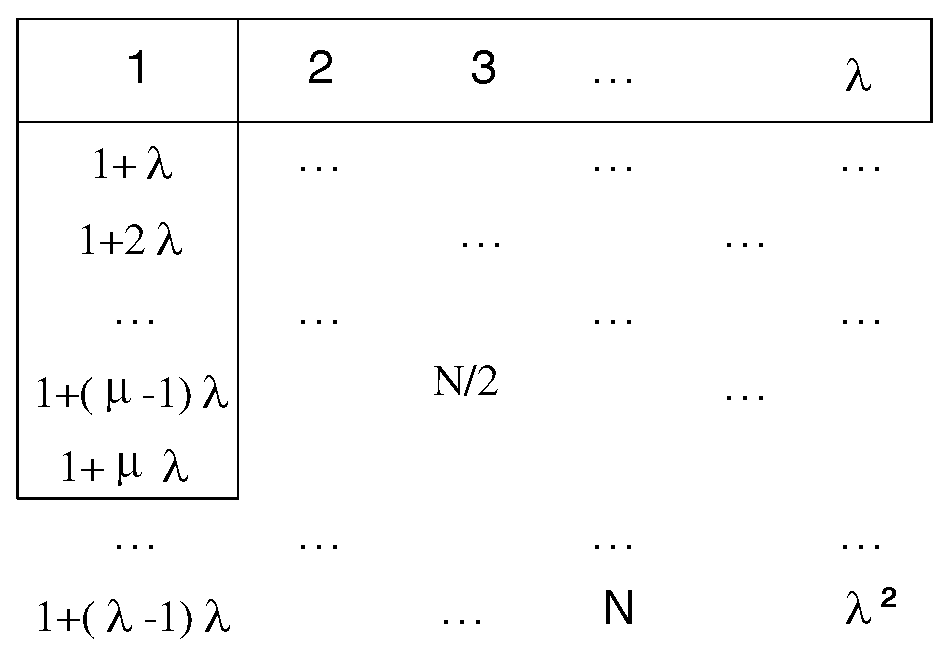
\includegraphics[width=2in]{./Figure/matrix}
\caption{An Sketch of RDS construction in Alg. \ref{RDS}}
\label{matrix}
\end{figure}


%The correctness proof of the construction
\begin{lemma}
\label{RDS1}
Set $R = \{r_0, r_1, ..., r_{\lambda + \mu - 1}\}$ constructed in Alg. \ref{RDS} is a RDS,
where $|R| = \lambda + \mu = \lceil \sqrt{N}  \rceil + \lceil \frac{\lceil \sqrt{N} \rceil}{2} \rceil
\approx \lceil \frac{3\sqrt{N}}{2}  \rceil$.
\end{lemma}


\begin{IEEEproof}
Obviously, if there exists one ordered pair $(a_i,a_j)$ satisfying  $a_i - a_j \equiv d$ (mod $N$),
an opposing pair $(a_j,a_i)$ exists such that
$a_j - a_i \equiv (N-d)$ (mod $N$). Thus we only need to find
at least one ordered pair $(a_i,a_j)$ for each $d \in [1, \lfloor N/2 \rfloor]$.

In the construction, $\lambda$ in Line \ref{RDSline1} is the smallest integer satisfying
$\lambda^2 \geq N$. Every $d$ within range $[1, \lfloor N/2 \rfloor]$
can be represented as: $ d = 1 + j \times \lambda - i$, where $1 \leq j \leq \mu,
1 \leq i \leq \lambda$. Thus, there exists $a_j = 1 + j \times \lambda$
from Line. \ref{RDSline2} and $a_i = i$ from Line. \ref{RDSline3}
satisfying  $a_j - a_i \equiv d$. Then, the lemma can be derived.
\end{IEEEproof}


%RDS Based Alano Algorithm
For symmetric nodes with duty cycle $\theta$, we present a RDS based Alano (RDS-Alano) algorithm as Alg. \ref{RDS-ND}.

In Alg. \ref{RDS-ND}, RDS is used to construct a deterministic
schedule for a node to turn on its radio in every period of length $T$,
and Alano is utilized as a probabilistic strategy to
determine whether it is in transmitting state or listening state.

\begin{algorithm}
\caption{RDS Based Alano Algorithm}
\label{RDS-ND}
\begin{algorithmic}[1]
\STATE $T := \lceil \frac{9}{4\theta^{2}} \rceil$; $t := 0$;
\STATE Invoke Alg. \ref{RDS} to construct the RDS $R = {r_0, r_1, ...,r_{\lceil \frac{3\sqrt{T}}{2}  \rceil}}$ under $Z_T$;
\WHILE {$True$}
   	 \IF{$(t + 1) \in R$}
    		\STATE Invoke Alg. \ref{Alano} to determine transmission state;
	\ELSE
    		\STATE Sleep;
	\ENDIF
	\STATE t := (t + 1) \% T;
\ENDWHILE
\end{algorithmic}
\end{algorithm}

%The time bound analysis   dutycycle zhengming

We derive discovery latency bound for RDS-Alano:

\begin{theorem}
\label{theoremRDS}
RDS-Alano guarantees that the discovery latency of a node
is bounded within $O(\frac{n\log n}{\theta^2})$ with high probability.
\end{theorem}

\begin{IEEEproof}
First, we verity that the duty cycle in RDS-Alano (denote as $\widetilde{\theta}$) is
$$
\widetilde{\theta} = \frac{|RDS|}{|T|} = \frac{\lceil \frac{3\sqrt{T}}{2}  \rceil}{T} = \theta.
$$

For any pair of neighbor nodes ($u_i$, $u_j$),
we can find an ordered pair ($r_i$, $r_j$) from their respective RDS
such that $r_i - r_j \equiv \delta_{ij}$ (mode $T$), where $\delta_{ij}$ is the time drift.
This implies any neighbor nodes can turn on their radios in the same time slot for at least once during every period of length $T$. 
Considering each period of $T$ time slots to be a `super' slot of Alano algorithm, we can derive that the discovery latency is bounded within $O(\frac{n\ln n}{\theta^2})$ slots with high probability by combining the analysis of Alano.
\end{IEEEproof}

\begin{remark}
In a RDS, a node can discovery its neighbors in different time slots. When treating a period of $T$ as a  `super' slot of Alano, 
there may be less than the total neighbors in each wake-up sub-slot,
resulting less collisions and lower latency compared to when all the neighbors wake up in the same sub-slot.
Thus the latency bound can not be larger.
\end{remark}


\subsection{TP-Alano for Asymmetric Nodes}


%Consider Local Duty Circle
Considering a more practical network where nodes can adjust their duty cycles, we present a traversing pointer method to synchronize time slots that nodes are in transmitting or listening state for asymmetric nodes.


For a more practical scenario, the nodes in a wireless sensor networks
for instance, are assigned to diverse tasks such as temperature measurement,
sunshine collection, etc., and thus ought to have asymmetric capability of
battery-management with local duty cycle $\theta_i$.

Suppose the duty cycle of node $u_i$ is $\theta_i$, we present a traversing pointer based Alano (TP-Alano) algorithm as Alg. \ref{P-ND}.
In each period of $T$ slots, a node turns on its radio in two different time slots, one of which is the
first slot of each period and the other one is a traversing slot that changes from period to period (as described in Line. \ref{P-NDline1}).

%Prime Based Neighbor Discovery Algorithm
\begin{algorithm}[!h]
\caption{Traversing Pointer Based Alano Algorithm}
\label{P-ND}
\begin{algorithmic}[1]
\STATE $T :=$ the smallest prime no less than $\frac{2}{\theta_i}$; $t := 0$;
\WHILE {$True$}
	\STATE $t_1 := t \% T$;
	\STATE $t_2 : =\lfloor t / T \rfloor \% (T - 1) +1$;\label{P-NDline1}
   	 \IF{$t_1 = 0~or~t_1 = t_2$}
    		\STATE Invoke Alg. \ref{Alano} to determine transmission state;
	\ELSE
    		\STATE Sleep;
	\ENDIF
	\STATE $t := t + 1$;
\ENDWHILE
\end{algorithmic}
\end{algorithm}

We call the first time slot of each period as \emph{fixed pointer} and the traversing
slot as \emph{traversing point}. The pointers are designed to guarantee that nodes $u_i, u_j$
could turn on their radio simultaneously in very period of length $T_i T_j$. A sketch of the pointers is described in Fig. \ref{TP}.

Note that, a period of $T$ slots is constructed as Line 1 where we try to \emph{find the smallest prime $\geq \frac{2}{\theta_i}$},
then it is likely to make the duty cycle of each period smaller than the expected one. This can be easily solved by selecting some random slots to turn on the radio for listening in each period $T$, to conform to the expected duty cycle.


\begin{figure}[!h]
\centering
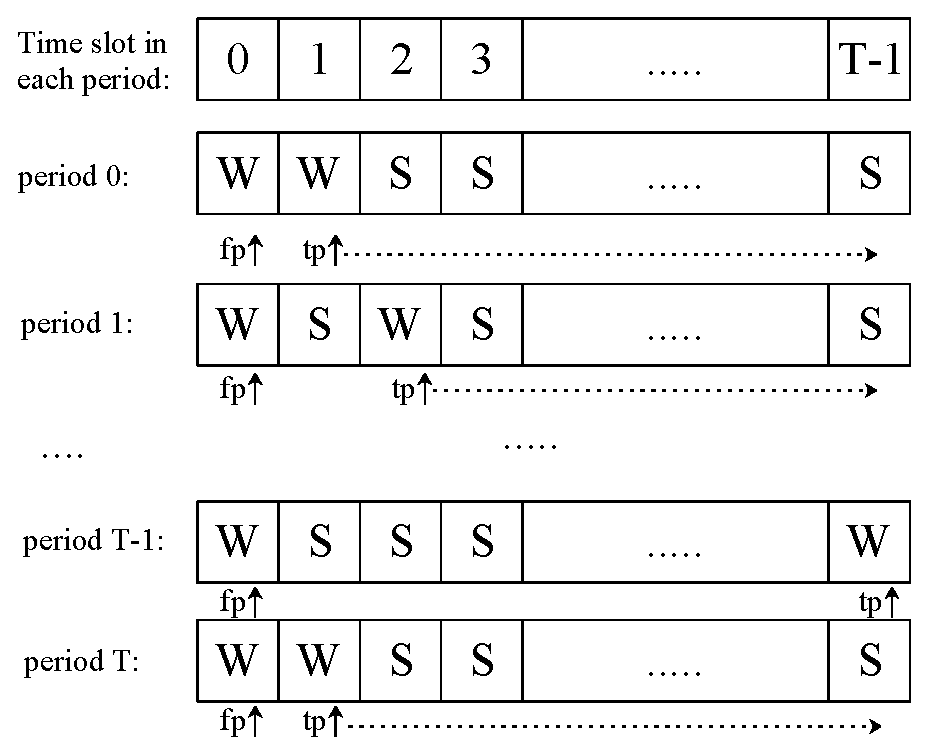
\includegraphics[width=3in]{./Figure/TP}
\caption{A sketch of TP construction in Alg. \ref{P-ND}}
\label{TP}
\end{figure}

%The correctness proof of the construction and the time bound analysis
We show the discovery latency of TP-Alano algorithm as:


\begin{theorem}
\label{PBND1}
TP-Alano guarantees that the discovery latency $L(i,j)$
is bounded within $O(\frac{nlogn}{\theta_i\theta_j})$ with high probability.,
where $\theta_i$ and $\theta_j$ are the duty cycles of
a pair of neighbors ($u_i$, $u_j$) respectively.
\end{theorem}



\begin{IEEEproof}
We first prove that any pair of nodes ($u_i$, $u_j$) turn on their radios (for transmitting or listening) simultaneously for at least once in every period of length $T_iT_j$.

\textbf{Case 1: $T_i \neq T_j$}. Since $T_i$ and $T_j$ are different primes,
according to Chinese Remainder Theorem\cite{ding1996chinese}, there exists a time slot $t_\tau \in \lbrack 0,T_iT_j ) $ satisfying:
\begin{equation}
\label{case1.1}
0 = t_\tau  \quad mod \quad  T_i.
\end{equation}
\begin{equation}
\label{case1.2}
\delta_{ij} = t_\tau  \quad mod \quad  T_j.
\end{equation}

Thus, there exists a fixed pointer of node $u_i$
and a fixed pointer of node $u_j$ in which both nodes turn on the radios in every period of length $T_iT_j$  .

\textbf{Case 2: $T_i = T_j$}. Since $T_i = T_j = T$, if the time drift between $u_i$ and $u_j$ is $\delta_{ij} = 0$, the fixed pointers of $u_i$ and $u_j$ will be the same in every period of length $T$.
Otherwise, since the traversing point will traverse all the time slots once during period of length $(T-1)T$,
there exists a traversing point of $u_i$ and a fixed pointer
of $u_j$ satisfying that both nodes turn on the radios simultaneously in every period of length $(T-1)T$; similarly a traversing point of $u_j$ and a fixed pointer of $i$ satisfying that they both turn on the radios.

Thus for any pair of neighbor nodes ($u_i$, $u_j$), they turn on their radios for transmitting or listening for at least once in every period of length $T_iT_j$. Considering
the whole period $T_iT_j$ to be a `super' slot of Alano, we derive that the discovery latency is bounded within $O(\frac{n\ln n}{\theta_i\theta_j})$ with high probability.
\end{IEEEproof}








% Evaluation
\section{Evaluation}
\label{Evaluation}

In this section, we experimentally verify our basic analysis
Then we evaluate the algorithms in simulated large-scale networks.

\subsection{Experiments for Fundamental Observation}

In our experiments, we implemented $16$ EZ$240$ sensors \cite{huang2012easipled}, each of which uses $8$MHz MSP$430$F$1611$ 
as the microprocessor and is equipped with $10$K RAM, 
$48$K ROM and $1$ M Flash. CC$2420$ is used as the communication 
module with the IEEE $802.15.4$ protocol. RTIMER\_ARCH\_CECOND is the clock frequency 
and a time slot is set as 500/RTIMER\_ARCH\_CECOND,
which is around $0.5$ms in the real world. As discussed in section \ref{RW}, the time slot of beacon-based 
algorithms, e.g. searchlight~\cite{bakht2012searchlight}, is set as $20$ms.
From the code in the MAC layer we can see  that CSMA mechanism makes the process to wait a random time 
when a collision happens, which implies that collisions result in a high latency.    

\begin{table}[htbp]
\caption{Experimental results of discovery latency}
\centering
\begin{tabular}{|l|c|c|c|c|} 
\hline
\textbf{Algorithms} & \textbf{Alano} & \textbf{Hedis} & \textbf{Searchlight} & \textbf{ALOHA} \\
\hline
\textbf{Average latency} & \textbf{$1.278$} & \textbf{$1.847$} & \textbf{$8.58$} & \textbf{$10.07$} \\
\hline
\textbf{Maximum latency} & \textbf{$1.52$} & \textbf{$3.11$} & \textbf{$10.11$} & \textbf{$16.13$} \\
\hline
\textbf{Minimum latency} & \textbf{$1.10$} & \textbf{$0.73$} & \textbf{$6.31$} & \textbf{$5.11$} \\
\hline
\end{tabular}
\label{Exp}
\end{table}

We compared Alano with Searchlight~\cite{bakht2012searchlight}, Hedis~\cite{chen2015heterogeneous}
and Aloha-like~\cite{you2011aloha} in the experiments. The result in the Table \ref{Exp} shows that Alano outperforms the other algorithms.
Hedis shows a low latency which results from it's ideal latency bound for two nodes, its weakness in handling collisions is not obvious in small scale networks. 
However, as the number of neighbors increase, collisions of Hedis \cite{chen2015heterogeneous} increased to the tune of 10.1\% to 19.96\%.
Searchlight is a typical beacon-based algorithm with a larger time slot, which results in high latency.
Aloha-like is designed for a clique network and the probability adopted is not optimal.


\subsection{Simulations for energy-restricted Large-scale Networks}


To simulate a large-scale network, we implemented Alano in C++ and evaluated the algorithms in a cluster of 9 servers,
each equipped with an Intel Xeon 2.6GHz CPU with 24 hyper-threading cores, 64GB memory and 1T SSD.

We simulated a network that follows uniform distribution and Gaussian distribution respectively.
For uniform distribution, we suppose $500$ nodes are distributed in an area of $100m \times 100m$ 
and each node's communication range is $\Delta = 10m$. For Gaussian distribution, we suppose 
$1000$ nodes are distributed in the same area, but each node's communication range is $\Delta = 5m$. 
We set the Gaussian distribution to $N(50,15^2)$ in our evaluation.
We set the duty cycle of a node to be $0.1$ for symmetric nodes; 
for asymmetric nodes, we set their duty cycle randomly from $0.05$ to $0.15$ with step $0.02$.
These settings make the network more complicated and realistic than that in
\cite{wang2015blinddate, sun2014hello, bakht2012searchlight,
chen2015heterogeneous, kandhalu2010u, you2011aloha,
mcglynn2001birthday, song2014probabilistic, vasudevan2009neighbor}.


We evaluated Alano, Aloha-like~\cite{you2011aloha}, Hello~\cite{sun2014hello}, Hedis~\cite{chen2015heterogeneous}, and Searchlight~\cite{bakht2012searchlight} in the generated networks. %Besides, we evaluated G-Nihao(we choose the best parameters, $m=n$, $\alpha=0.054$)~\cite{qiu2016talk}, but $500$ symmetric nodes in uniform distribution can only discover $2\%$ neighbors, which is worse than other $3$ deterministic algorithms we choose. Thus, we didn't show its result in our figures.
%Hedis only has two states $\{ON, OFF\}$ (representing the radio is on or off). To make the comparison more fair, we assume that when a node is in $\{ON\}$ state, it transmits or listens with equal probability $0.5$. 
Hello and Searchlight has a beacon transmission of $0.54ms$ at the beginning and end of each slot, and a beacon makes up about $1/40$ of a slot, so we divide each $\{ON\}$ slot into $40$ mini-slots, and the node transmits at the first and last mini-slot, and listens in other mini-slots.
In the following parts, we show that Alano has lower latency, higher discovery rate, and better scalability. %, and better robustness.




\subsubsection{Speed-Discovery Latency}

\begin{figure}[!h]
\centering
\subfigure[Uniform Distribution]{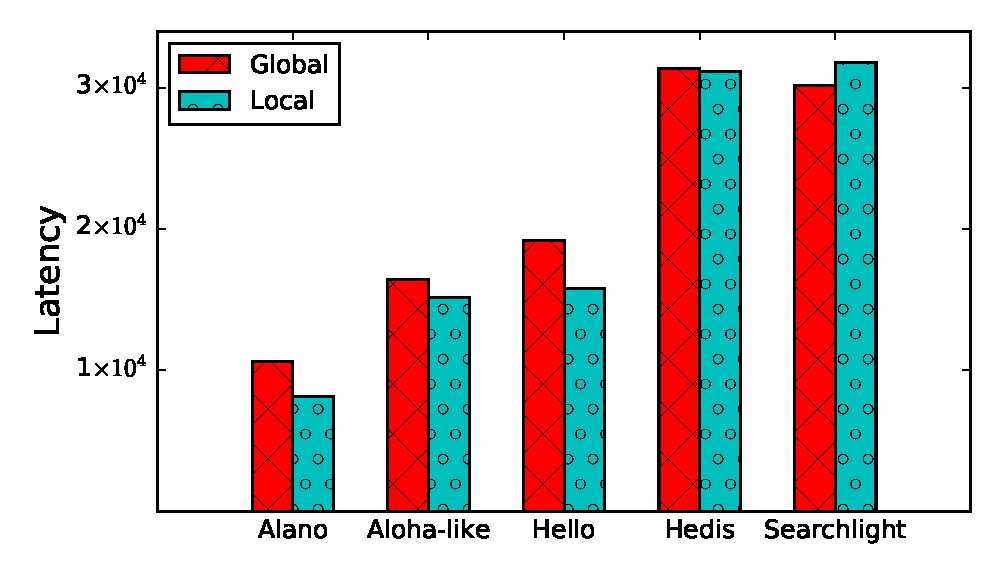
\includegraphics[width=1.65in]{Figure/latency_uniform}}
\hspace{0.01in}
\subfigure[Gaussian Distribution]{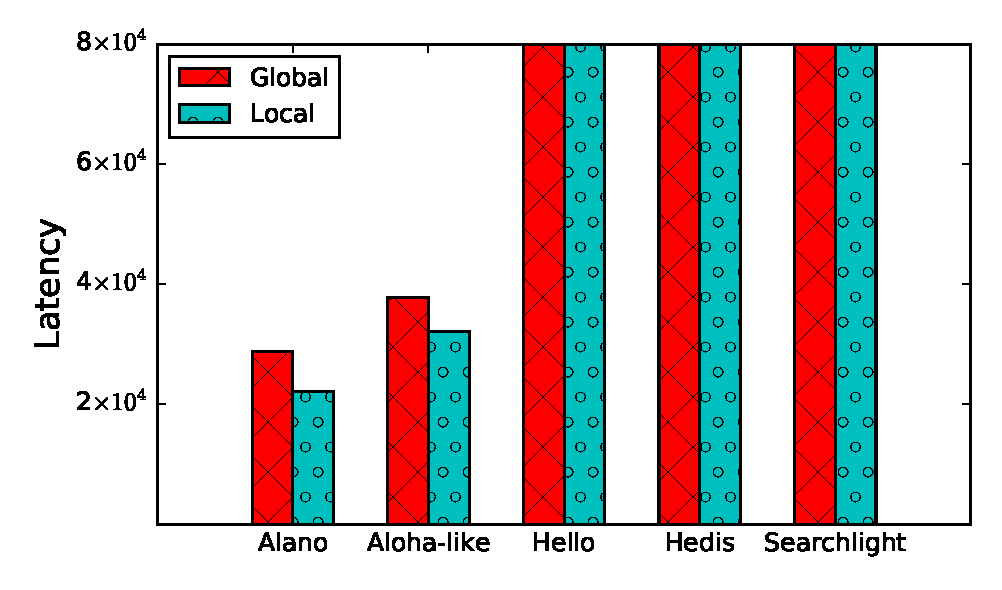
\includegraphics[width=1.65in]{Figure/latency_normal}}
\caption{Alano achieves lower latency.}
\label{fig_latency}
\end{figure}

When nodes follow uniform distribution, we show the discovery latency comparison for both symmetric nodes and asymmetric nodes in Fig. \ref{fig_latency}(a).
From the figure, Alano achieves $54.64\%$ to $1.95$ times lower discovery latency for symmetric nodes, and $85.25\%$ to $2.91$ times lower discovery latency for asymmetric nodes.
When nodes follow Gaussian distribution, as depicted in Fig. \ref{fig_latency}(b), 
Alano achieves $31.35\%$ to $1.21$ times lower discovery latency for symmetric nodes, 
and $45.94\%$ to $1.88$ times lower discovery latency for asymmetric nodes.
The deterministic algorithms, Hello, Hedis and Searchlight, have high latency due to either collisions or larger time slots. 


\subsubsection{Quality-Discovery Rate}

% \begin{figure}[!h]

% \subfigure[Uniform Distribution with Global Duty Cycle]{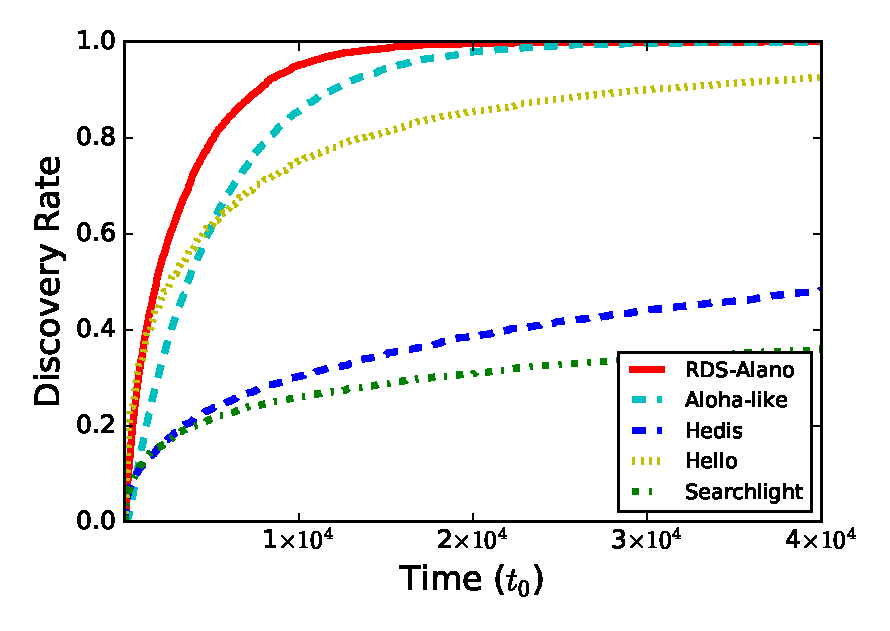
\includegraphics[width=1.65in]{Figure/rate_uniform}}
% \hspace{0.01in}
% \subfigure[Normal Distribution with Global Duty Cycle]{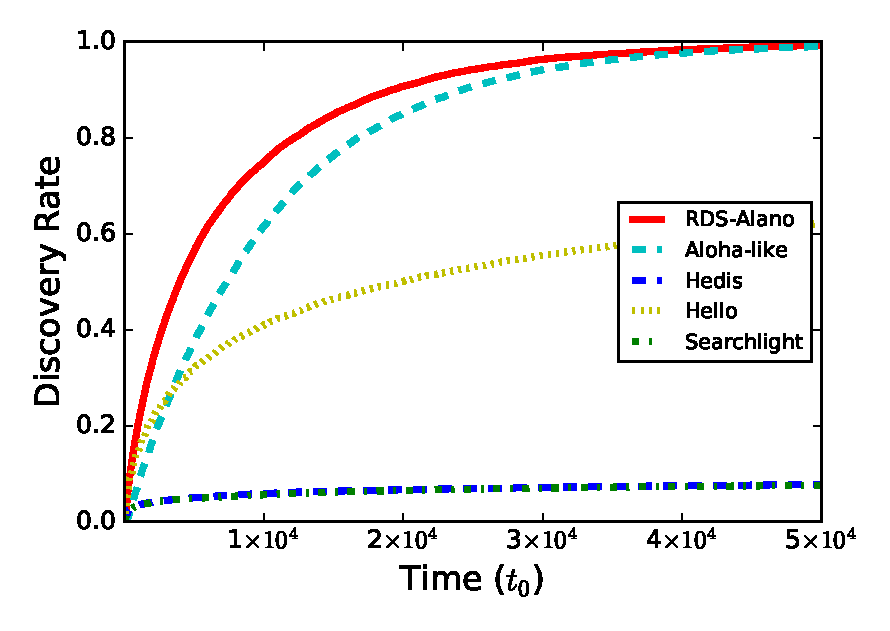
\includegraphics[width=1.65in]{Figure/rate_normal}}
% \hspace{0.01in}
% \subfigure[Uniform Distribution with Local Duty Cycle]{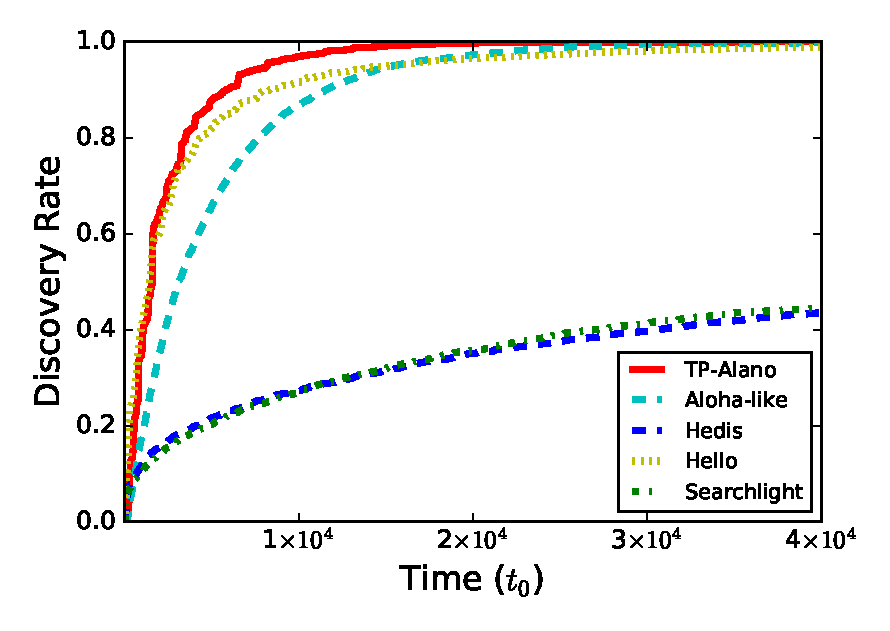
\includegraphics[width=1.65in]{Figure/rate_local_uniform}}
% \hspace{0.01in}
% \subfigure[Normal Distribution with Local Duty Cycle]{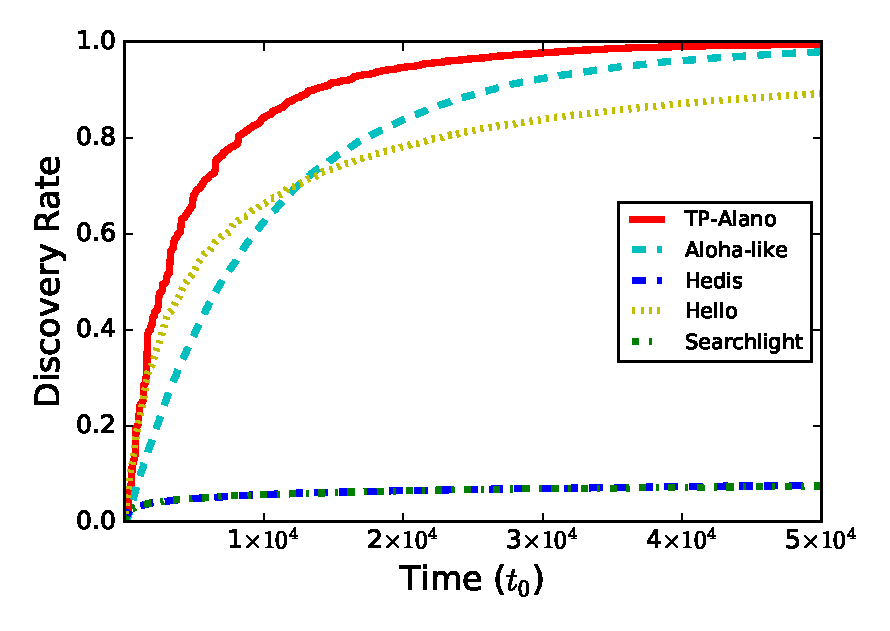
\includegraphics[width=1.65in]{Figure/rate_local_normal}}
% \caption{Alano achieves higher discovery rate.}
% \label{fig_timerate}
% \end{figure}


% Fig. \ref{fig_timerate} shows Alano with either global or local duty cycle, has higher discovery rate during the whole course of neighbor discovery in both uniform and normal distribution. The deterministic algorithms Hello, Hedis and Searchlight cannot discover all channels, because of the occurence of collisions. Aloha-like discovers more slowly than Alano when it has discovered a certain number of channels, such as $80\%$ channels in Uniform Distribution with Global Duty Cycle, because it is difficult for pure probabilistic algorithm to deal with the small amount of undiscovered neighbors.

\begin{figure}[!h]

\subfigure[Symmetric Nodes in Uniform Distribution]{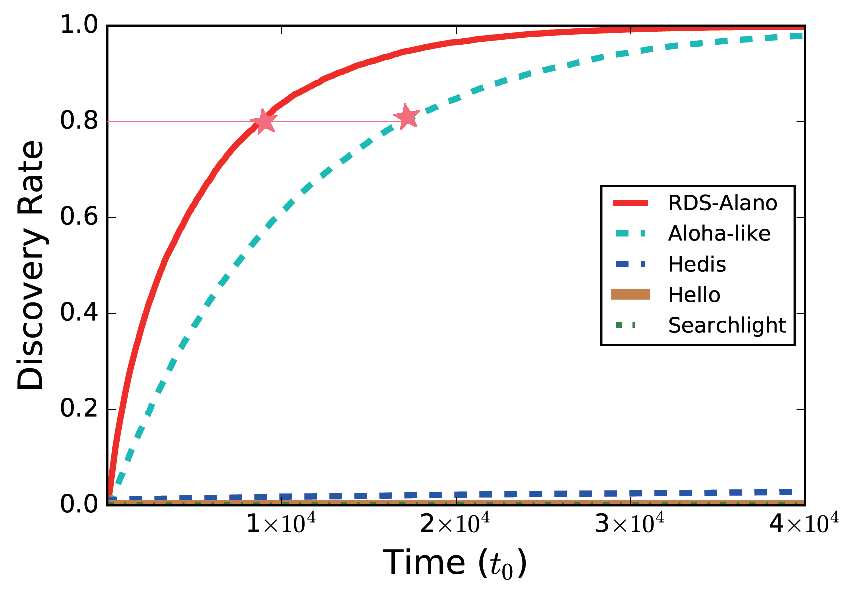
\includegraphics[width=1.65in]{Figure/rate_uniform1}}
\hspace{0.01in}
\subfigure[Symmetric Nodes in Gaussian Distribution]{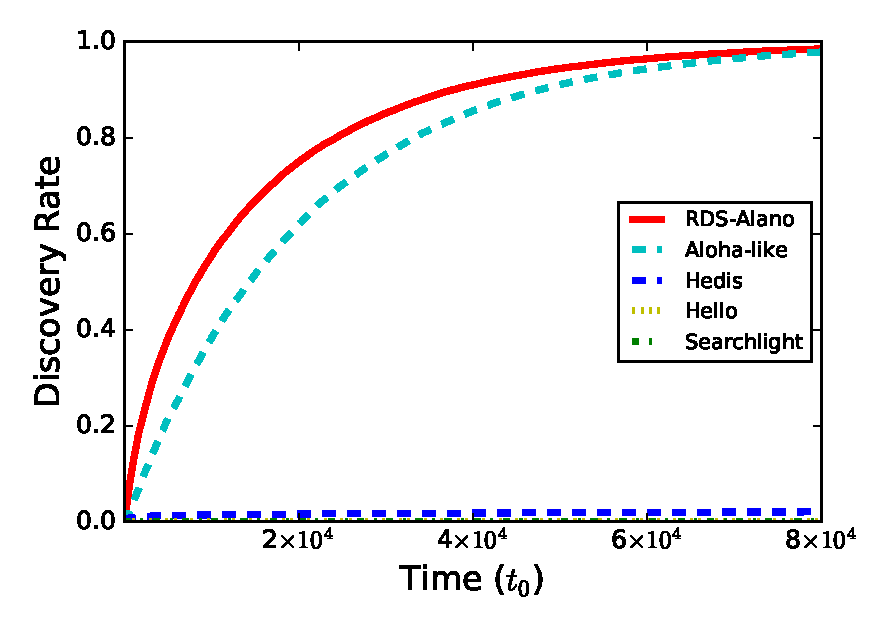
\includegraphics[width=1.65in]{Figure/rate_normal1}}
\hspace{0.01in}
\subfigure[Asymmetric Nodes in Uniform Distribution]{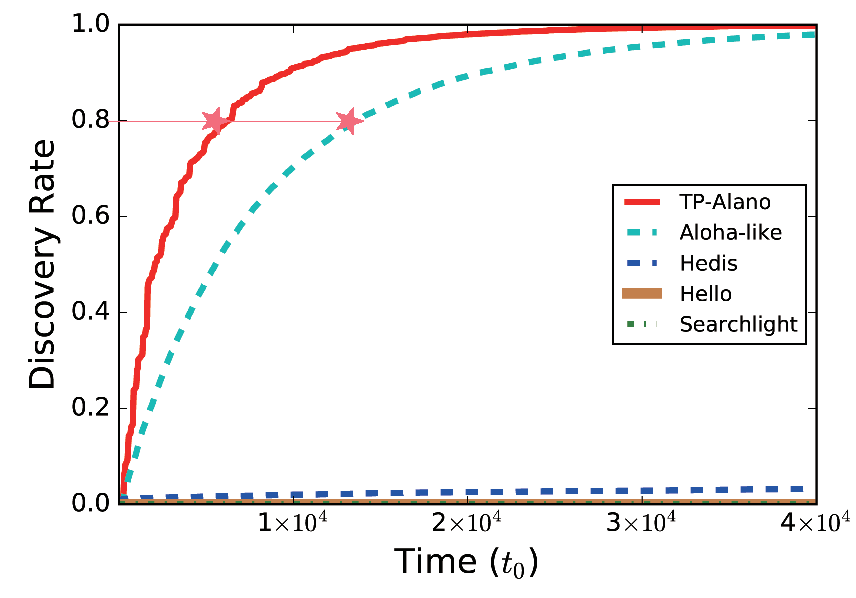
\includegraphics[width=1.65in]{Figure/rate_local_uniform1}}
\hspace{0.01in}
\subfigure[Asymmetric Nodes in Gaussian Distribution]{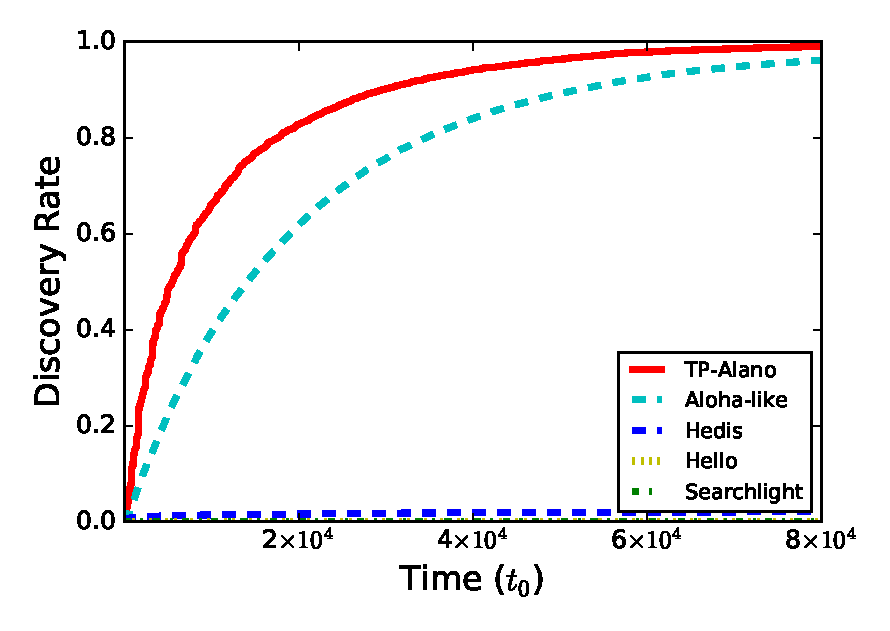
\includegraphics[width=1.65in]{Figure/rate_local_normal1}}
\caption{Alano achieves higher discovery rate.}
\label{fig_timerate_large}
\end{figure}


We use discovery rate to evaluate Alano's quality.
Discovery rate of a node $u_i$ is defined as the percentage of discovered neighbors over $u_i$'s all neighbors.
In Fig. \ref{fig_timerate_large}, we increase the number of nodes from $500$ to $1000$ for the uniform distribution, and increase the number of nodes from $1000$ to $2000$ for the Gaussian distribution, the results show that Alano has higher discovery rate during the whole process for both uniform and Gaussian distributions. It's remarkable that, the performance of Aloha-like is close to Alano in the Gaussian distribution. This is because a number of nodes gather around the center area which makes the network similar to a clique, and thus Aloha-like shows its strength.  
%Aloha-like discovers more slowly than Alano when it has discovered a certain number of channels, such as $80\%$ channels in Uniform Distribution with Global Duty Cycle, because it is difficult for pure probabilistic algorithm to deal with the small amount of  undiscovered neighbors.





\subsubsection{Scalability-Duty Cycle and Network Density}

We evaluated Alano's scalability regarding duty cycle and network density.

\begin{figure}[!h]
\centering
\subfigure[Uniform Distribution]{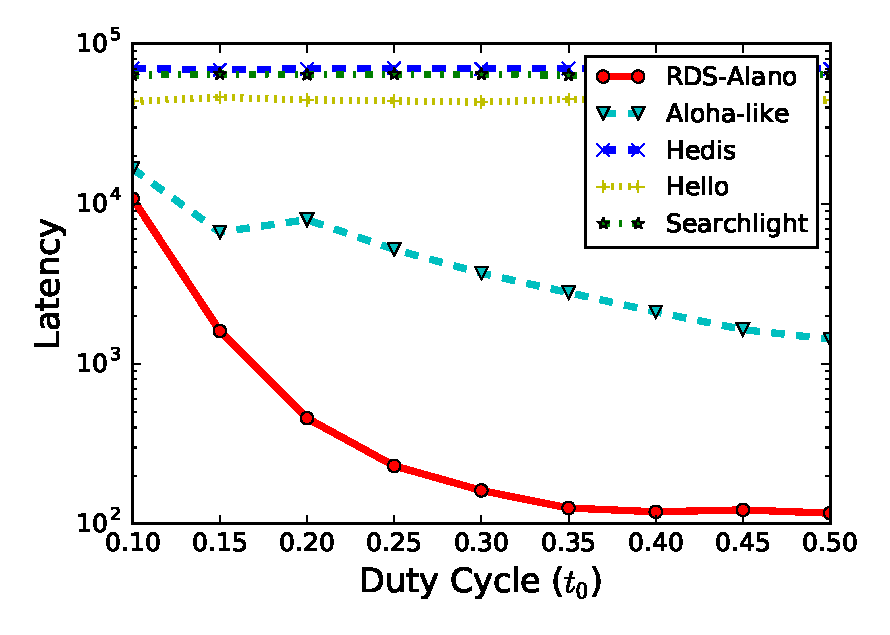
\includegraphics[width=1.65in]{Figure/dutycycle_uniform}}
\hspace{0.01in}
\subfigure[Gaussian Distribution]{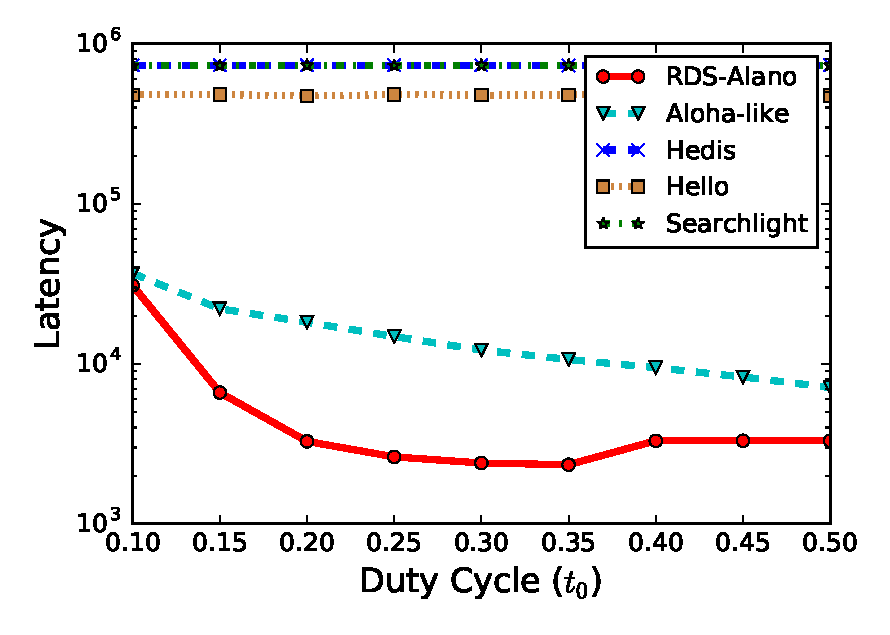
\includegraphics[width=1.65in]{Figure/dutycycle_normal}}
\caption{Alano achieves lower latency in different duty cycle.}
\label{fig_dutycycle}
\end{figure}


\emph{Duty Cycle.}
When symmetric nodes with different duty cycles, Fig. \ref{fig_dutycycle} shows that Alano has lower latency. Compared with Aloha, Alano has from $53.66\%$ to $11.23$ times lower latency. The latency of Alano and Aloha generally decreases as the duty cycle increases, while Hello, Hedis and Searchlight have high latency due to the collision. In Gaussian distribution, Alano has a small twist with respect to the duty cycle $0.35$, because when the duty cycle increases, nodes are more likely to transmit and therefore collide.


\begin{figure}[!h]
\centering
\subfigure[Uniform Distribution]{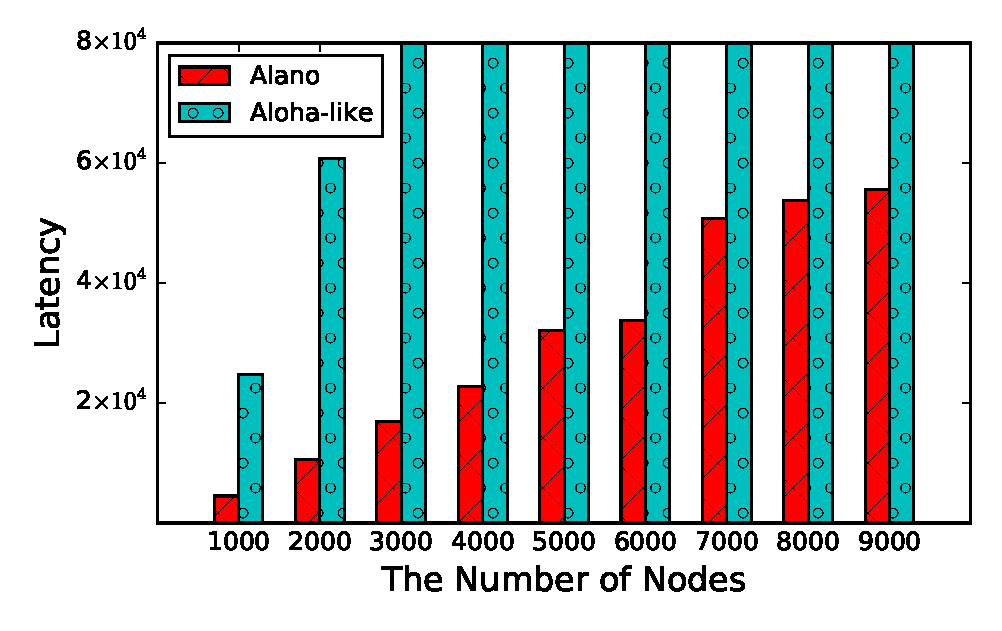
\includegraphics[width=1.65in]{Figure/node_uniform}}
\hspace{0.01in}
\subfigure[Gaussian Distribution]{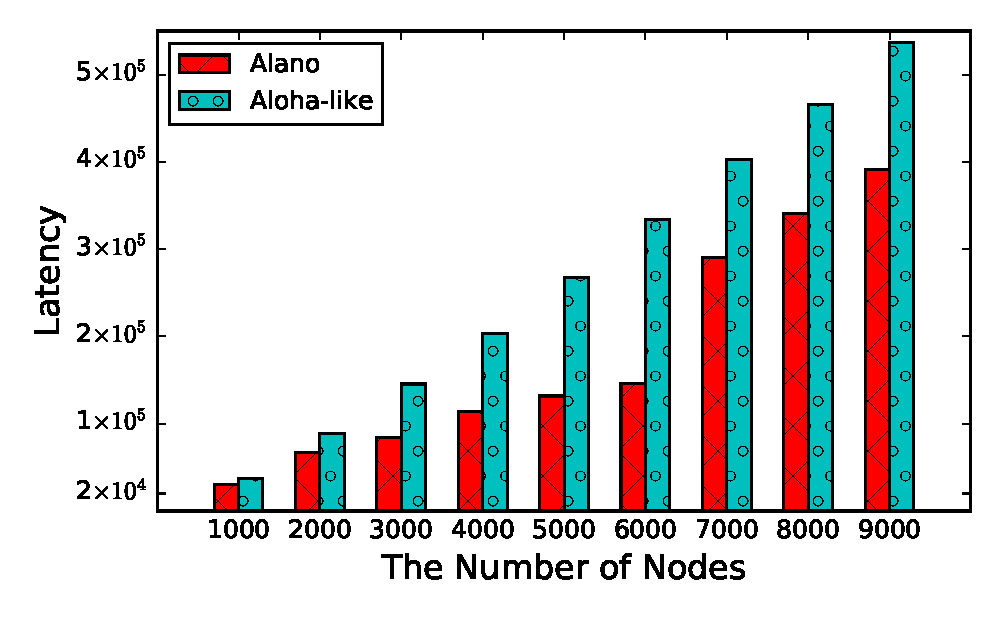
\includegraphics[width=1.65in]{Figure/node_normal}}
\caption{Alano achieves lower latency when the network becomes denser.}
\label{fig_node}
\end{figure}

\emph{Network Density.}
When the number of nodes increases, the network becomes denser. We choose Aloha-like algorithms for comparison because Hello, Hedis and Searchlight already have higher latency than Aloha-like when there are $500$ nodes in uniform distribution and $1000$ nodes in Gaussian distribution.
As shown in Fig. \ref{fig_node}(a), Alano achieves $4.68$ times to $6.51$ times lower discovery latency than Aloha-like algorithm for uniform distribution, when the number of nodes increases from $1000$ to $9000$.
When the number of nodes increases from $1000$ to $9000$ for Gaussian distribution, Alano achieves $25.23\%$ to $1.03$ times lower discovery latency as shown in Fig. \ref{fig_node}(b).  



% \subsection{Robustness}

% \begin{figure}[!h]
% \centering
% \subfigure[Uniform Distribution]{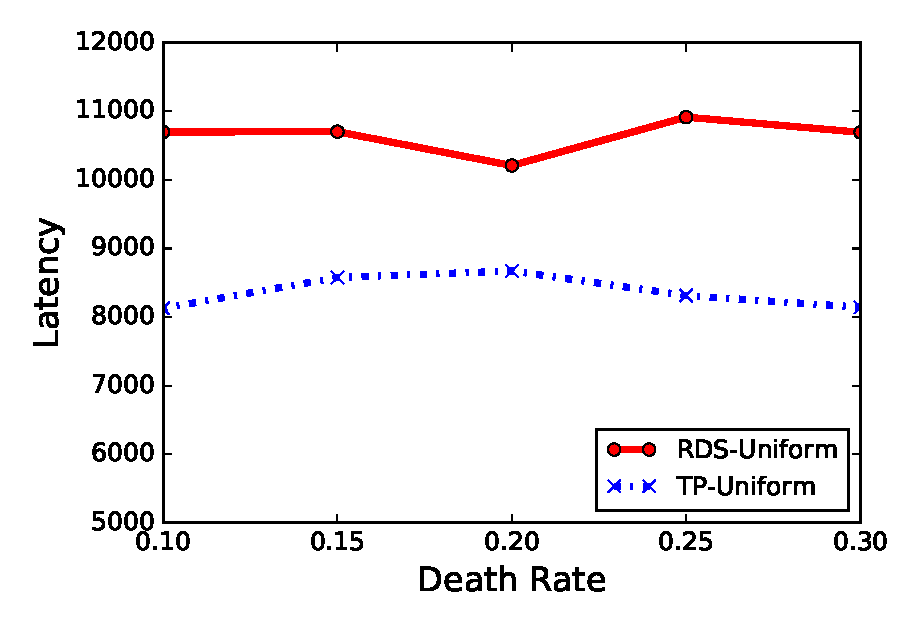
\includegraphics[width=1.65in]{Figure/robustU}}
% \hspace{0.01in}
% \subfigure[Gaussian Distribution]{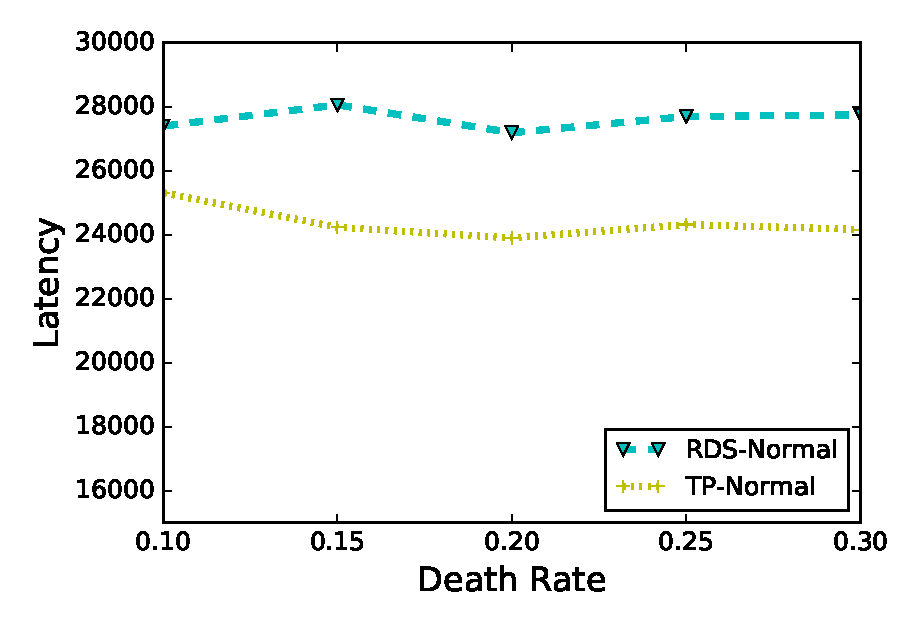
\includegraphics[width=1.65in]{Figure/robustN}}
% \caption{Alano still reaches low latency when nodes die.}
% \label{fig_robust}
% \end{figure}

% In reality, a node may leave the network now and then (such as the node runs out of energy or the node is offline for other usage). We evaluate the robustness of the neighbor discovery algorithms in Fig. \ref{fig_robust}. When $5\%$ to $30\%$ nodes die (see x-axis of the figure), Alano still reaches low discovery latency for both uniform and Gaussian distributions. %(?? others?)


%**To be deleted when the paper is done
(Note : Evaluation is expected to be around 1 page)
%**

% This section will talk about conclusion of the paper
\section{Conclusion}
\label{Conclusion}
The conclusion goes here.
With different duty cycle, Fig. 8 shows that Alano has lower latency. Compared with Aloha, Alano has from 53.66\% to 11.23 times lower latency. The latency of Alano and Aloha generally decreases as the duty cycle increases, while Hello, Hedis and Searchlight have high latency due to the collision. In normal distribution, Alano has a small twist with duty cycle 0.35, because when the duty cycle increases, nodes are more likely to transmit and therefore collide.

\bibliographystyle{IEEEtran}
\bibliography{ref}

%**To be deleted when the paper is done
\vspace{3mm}
(Note : Conclusion and Reference are expected to be less than 1 page)
%**


\end{document}


\grid